% ============================================================
% ============================================================
% NACA0012 -- SURFACE TEMPERATURE AND FREEZING FRACTION
% ============================================================
% ============================================================


% ============================================================
% AE3932
% ============================================================

\begin{frame}{\small NACA0012 -- Surface Temperature and Freezing Fraction -- AE3932}
\scriptsize

\begin{columns}[T,onlytextwidth]

\begin{column}{0.50\textwidth}
    \centering
    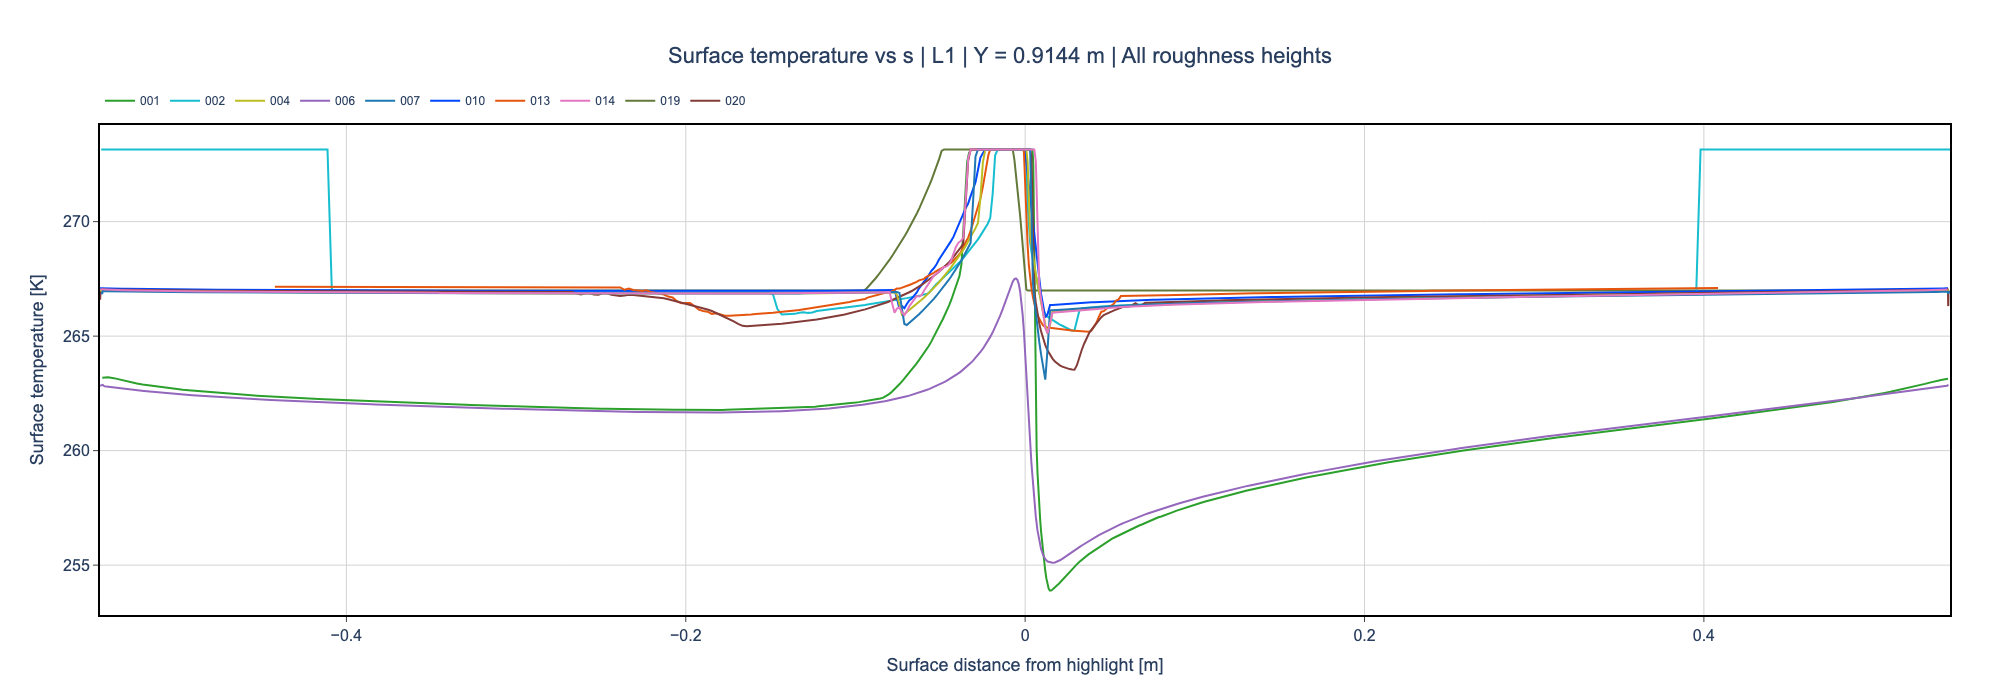
\includegraphics[width=\textwidth]{FIGURES/SURF_TEMP_FF/tc_naca0012_ae3932_L1_surface_temperature_vs_s_slice_0p9144_all_roughness.png}

    \vspace{0.05cm}

    {\scriptsize\textbf{Surface Temperature}}
\end{column}

\begin{column}{0.50\textwidth}
    \centering
    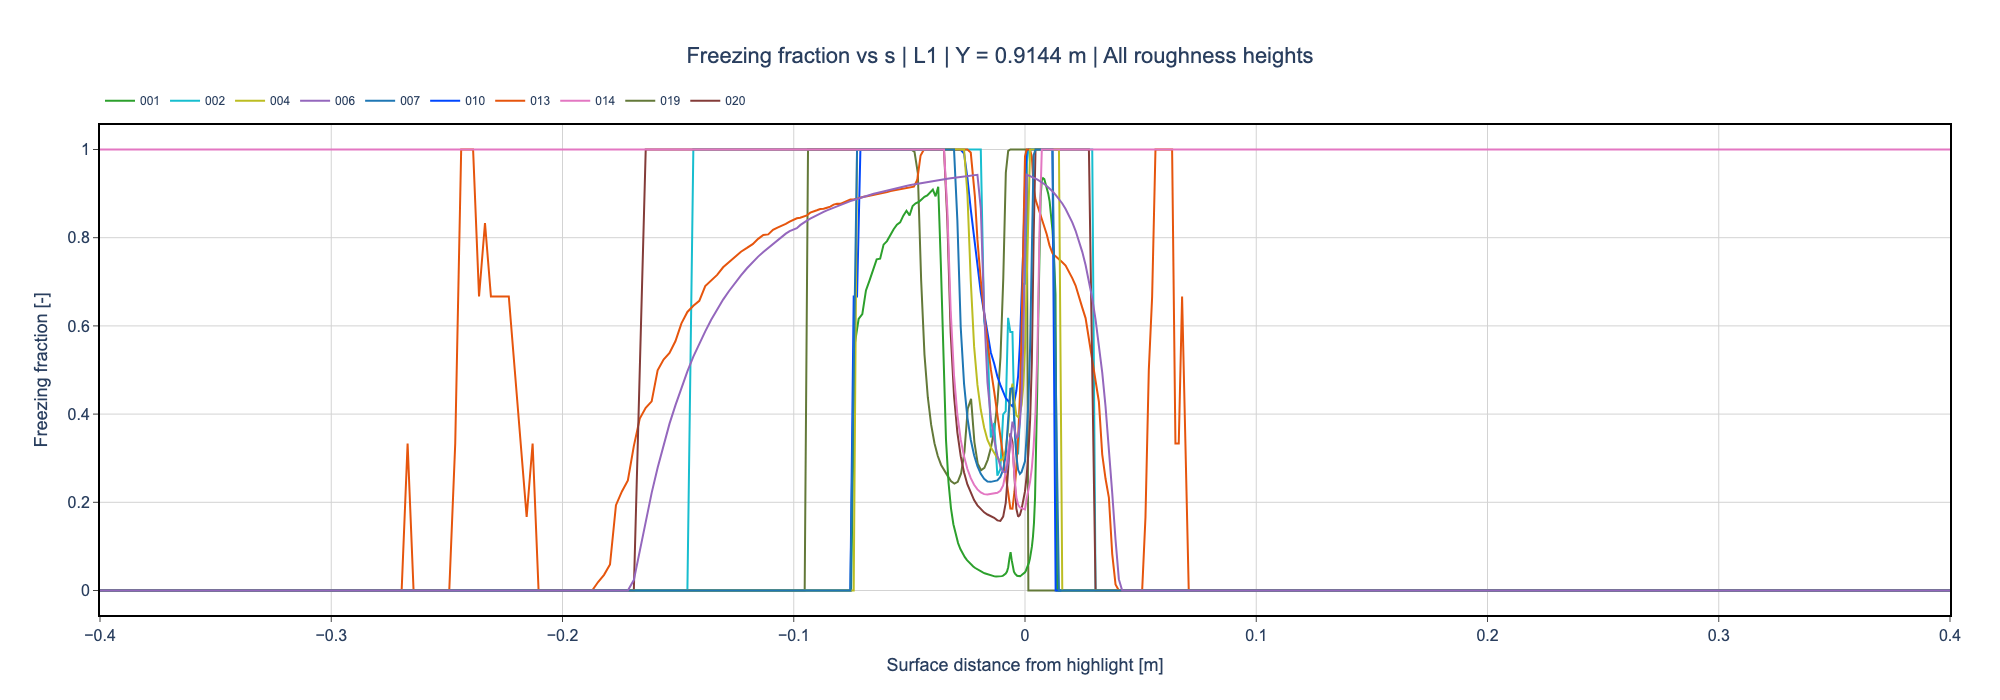
\includegraphics[width=\textwidth]{FIGURES/SURF_TEMP_FF/tc_naca0012_ae3932_L1_freezing_fraction_vs_s_slice_0p9144_all_roughness.png}

    \vspace{0.05cm}

    {\scriptsize\textbf{Freezing Fraction}}
\end{column}

\end{columns}

\vspace{0.15cm}

\begin{block}{\scriptsize Assessment}
\begin{itemize}
    \item Substantial code-to-code variability is observed in both the surface temperature and freezing-fraction distributions.
    \item The predicted freezing fraction exhibits different thermodynamic regimes and transition locations across submissions.
    \item These sharp and spatially shifted transitions make direct pointwise comparison of freezing fraction particularly difficult.
\end{itemize}
\end{block}

\end{frame}


% ============================================================
% AE3933
% ============================================================

\begin{frame}{\small NACA0012 -- Surface Temperature and Freezing Fraction -- AE3933}
\scriptsize

\begin{columns}[T,onlytextwidth]

\begin{column}{0.50\textwidth}
    \centering
    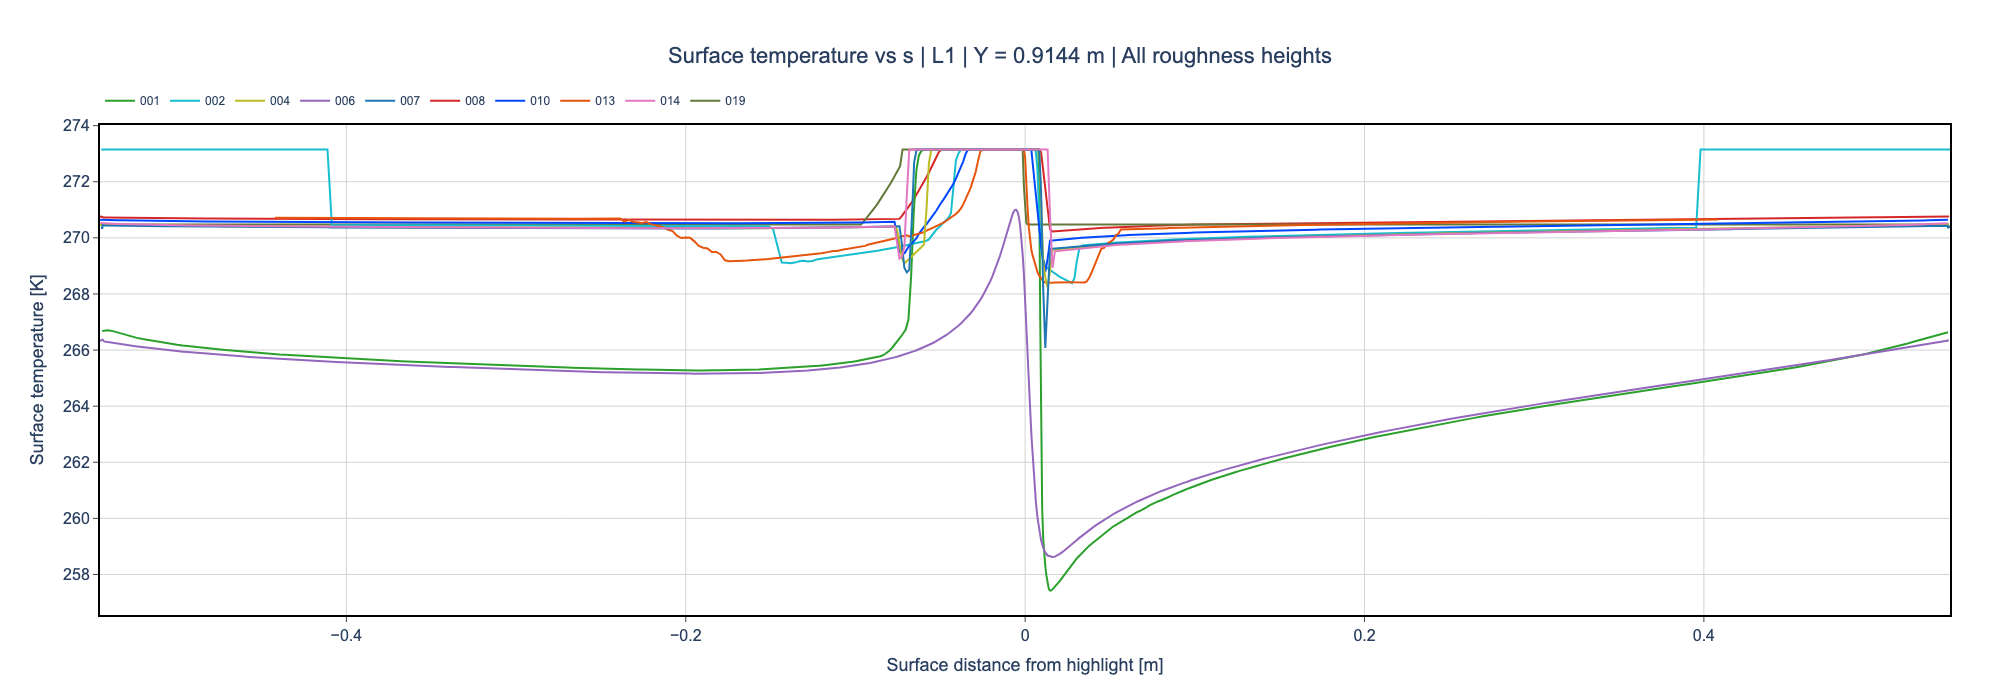
\includegraphics[width=\textwidth]{FIGURES/SURF_TEMP_FF/tc_naca0012_ae3933_L1_surface_temperature_vs_s_slice_0p9144_all_roughness.png}

    \vspace{0.05cm}

    {\scriptsize\textbf{Surface Temperature}}
\end{column}

\begin{column}{0.50\textwidth}
    \centering
    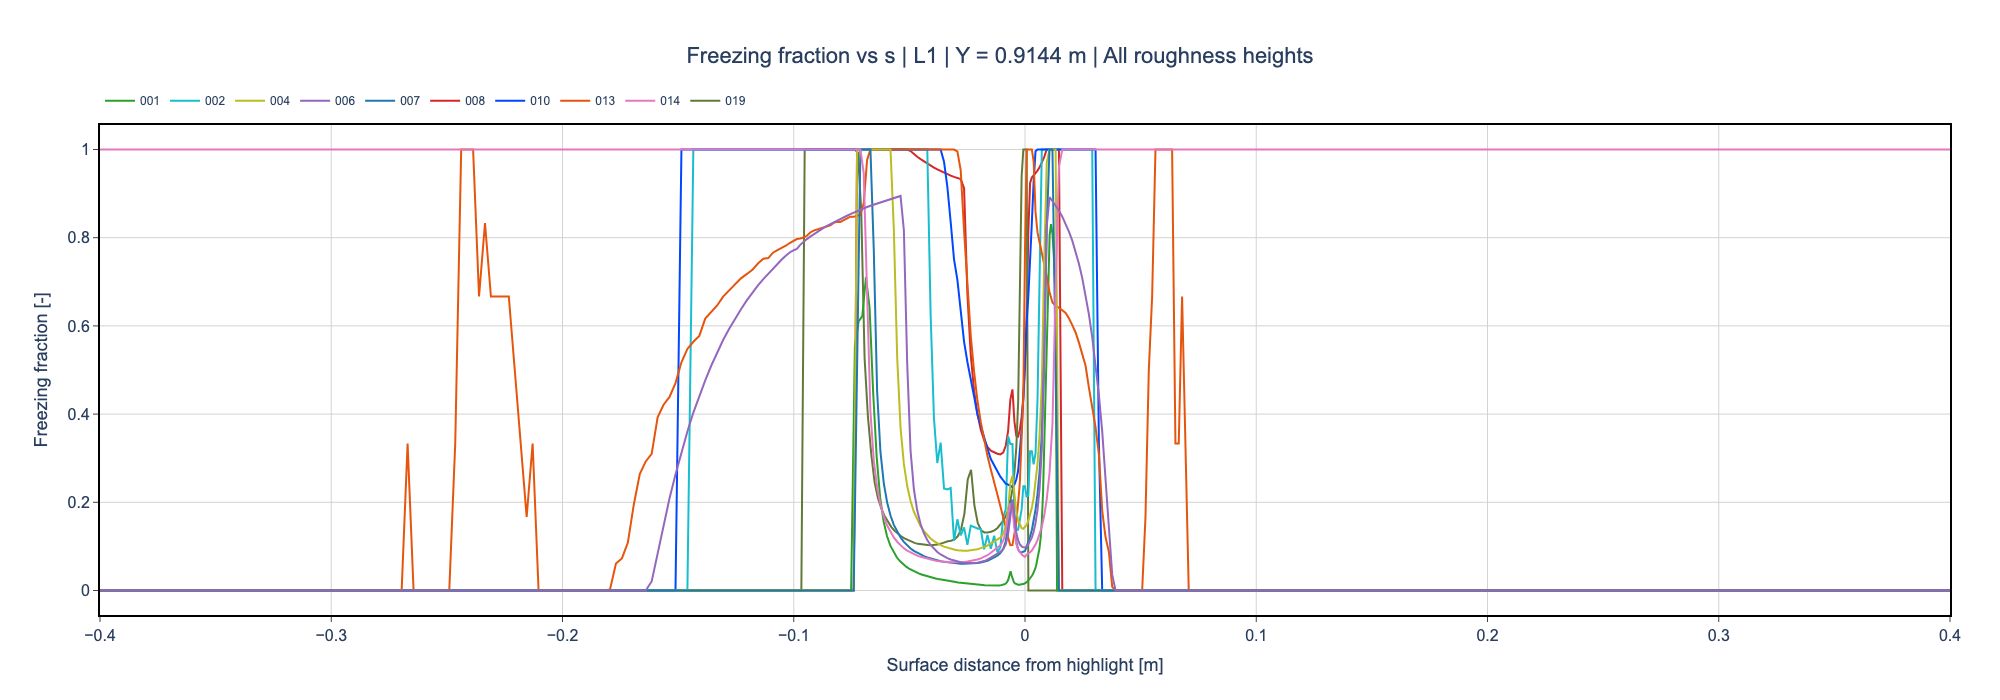
\includegraphics[width=\textwidth]{FIGURES/SURF_TEMP_FF/tc_naca0012_ae3933_L1_freezing_fraction_vs_s_slice_0p9144_all_roughness.png}

    \vspace{0.05cm}

    {\scriptsize\textbf{Freezing Fraction}}
\end{column}

\end{columns}

\vspace{0.15cm}

\begin{block}{\scriptsize Assessment}
\begin{itemize}
    \item Similar code-to-code variability is observed for AE3933, particularly in the extent and location of the different freezing regimes.
    \item Differences in surface temperature are accompanied by substantial differences in the predicted freezing-fraction distributions.
    \item As for AE3932, the discontinuous nature and spatial displacement of the freezing transitions make a direct pointwise statistical assessment difficult.
\end{itemize}
\end{block}

\end{frame}
